\documentclass[smaller,dvipsnames,ratio=169]{beamer}

\usetheme[numbering=fraction,%
          block=fill,%
          sectionpage=progressbar,%
          subsectionpage=progressbar,%
  ]{metropolis} % Use metropolis theme
\setbeamercovered{invisible}

\usepackage[utf8]{inputenc}
\usepackage{xcolor}
\usepackage{xspace}
\usepackage{booktabs}
\usepackage{amssymb}
\usepackage{listings}
\usepackage{todonotes}

\usepackage{tikz,comment}
\usetikzlibrary{shapes.multipart,positioning,backgrounds,positioning,fit,calc,arrows.meta}


\newcommand{\htw}{\emph{Hunt the Wumpus }}

\title{Hakuna Matata: A Logic-Based Agent for the \htw Game}
\subtitle{Team White}
\author{Filippo~De~Bortoli \and Aneta~Koleva \and Lorenz~Leutgeb}
\institute{Free University of Bozen-Bolzano\\[2mm] \texttt{\{\href{mailto:filippo.debortoli@stud-inf.unibz.it}{filippo.debortoli},\href{mailto:aneta.koleva@stud-inf.unibz.it}{aneta.koleva},\href{mailto:lorenz.leutgeb@stud-inf.unibz.it}{lorenz.leutgeb}\}\newline @stud-inf.unibz.it}}
\date{01.06.2018}

\begin{document}

  \maketitle

  \begin{frame}{Outline}
    \tableofcontents
  \end{frame}

  \section{Introduction}

  \begin{frame}{Task}
    \begin{enumerate}
      \item Develop an intelligent agent that plays the \htw game.
      \item Implement a strategy to complete the knowledge about the state of the world and to be able to reason with respect to it. 
      \item Find an optimal strategy, i.e. maximize score.
    \end{enumerate}
  \end{frame}
%not sure if a slide with explanation of the game is needed

  \begin{frame}{Tools of the Trade}
  \begin{enumerate}
    %\item Pragmatic choices to avoid any confusions
    %\item Keeping it DRY (Don't Repeat Yourself)
    %\item Avoid reinvention
    \item Simulator rewritten in Python 3.6 (removes C dependency)
  \end{enumerate}

  \begin{center}
  \begin{tabular}{lll}
    \textbf{Tool/Library} & \textbf{Version} & \textbf{Purpose} \\
    Python & 3.6 & Runtime \\
    PyTest & 3.0 & Benchmarking \\
    DLV & Dec 2012 & ASP Solver \\
    networkX & 2.1 & Graph management \\
    ? & ? & Dependency management \\
  \end{tabular}
  \end{center}
  \end{frame}

  \section{Ideas and used concepts}

\begin{comment}
  \begin{frame}{Hybrid Agent}
  	
      \begin{tabular}{lll}
        \textbf{Component} & \textbf{Task} & \textbf{Language} \\
        Perceptor & Retrieves what is perceived in current location & Python \\
        Long-term Memory & Stores information about what has been discovered and done & Python \\
        Action Graph & Searches for optimal actions to be taken & Python \\
        Working Memory & Stores information needed to decide next action & Python \\
        Planner & Infers new knowledge and decides next action & ASP \\ 
      \end{tabular}
  
  \end{frame}
   
\end{comment}


 \begin{frame}{World Knowledge}
	
	  \begin{itemize}
		\item Static, partly-observable environment.
		\item Incomplete initial knowledge.
		\item Safety first!
		\item Discovers size of the world when it bumps. 
		\item Dangers and how to reason to avoid them. 
	  \end{itemize}
 \end{frame}

 \begin{frame}{Why ASP and DLV?}
	\begin{itemize}
		\item Previous experience with ASP.
		\item Allows to model non-monotonic reasoning through CWA. 
		\item Combines a high-level
		logic with grounding and solving. 
		\item DLV allows processing of incomplete knoledge. 
		\item At each time step, ASP solver called after perception has been caught.
		
	\end{itemize}
 \end{frame}

  \begin{frame}{$A^{\star}$ Search and World Exploration}
	 \begin{itemize}
	 	\item Build a reachability graph such that:
		 	\begin{itemize}
				 \item Vertices are all the safe and reachable rooms that still haven't been explored.
				 \item Edges are the connections between these rooms.
		    \end{itemize}
	    \item Calculate the weights using the cost function: 
	    $$
	    g(C,C^\prime) := M((X,Y),(X^\prime,Y^\prime)) + R(O,O^\prime)
	    $$
	    % not sure if we should add more about the cost funstion here
	    \item Compute the minimal cost of reaching the target room using \emph{$A^{\star}$ search} : 
	    \(f(n) = g(n) + h(n)\)
	    \item Deciding a goal cell depending on the current mode of the agent .
	    \item Choosing next cell depending on the goal one.
		 
	 \end{itemize}
  \end{frame}

\begin{frame}{Cost graph example}
	\begin{figure}\centering
		\begin{tikzpicture}[roundnode/.style={circle, draw=black!60, very thick,minimum size=4mm}]
	\begin{scope}
		\node[regular polygon, regular polygon sides=4, align=center, text width={width("$(x + 1, y + 1)$")}] (n11) {$(x, y)$};
		\node[roundnode] (u11) [above=-1mm of n11] {$u$};
		\node[roundnode] (l11) [left=-1mm of n11] {$l$};
		\node[roundnode] (r11) [right=-1mm of n11] {$r$};
		\node[roundnode] (d11) [below=-1mm of n11] {$d$};
		\draw [<->] (u11) -> (l11);
		\draw [<->] (u11) -> (r11);
		\draw [<->] (d11) -> (l11);
		\draw [<->] (d11) -> (r11);
	\end{scope}
		
	\begin{scope}[xshift=5.1cm]
		\node[regular polygon, regular polygon sides=4, align=center, text width={width("$(x + 1, y + 1)$")}] (n21) {$(x + 1, y)$};
		\node[roundnode] (u21) [above=-1mm of n21] {$u$};
		\node[roundnode] (l21) [left=-1mm of n21] {$l$};
		\node[roundnode] (r21) [right=-1mm of n21] {$r$};
		\node[roundnode] (d21) [below=-1mm of n21] {$d$};
		\draw [<->] (u21) -> (l21);
		\draw [<->] (u21) -> (r21);
		\draw [<->] (d21) -> (l21);
		\draw [<->] (d21) -> (r21);
	\end{scope}
		
	\begin{scope}[yshift=5.2cm]
		\node[regular polygon, regular polygon sides=4, align=center, text width={width("$(x + 1, y + 1)$")}] (n12) {$(x, y + 1)$};
		\node[roundnode] (u12) [above=-1mm of n12] {$u$};
		\node[roundnode] (l12) [left=-1mm of n12] {$l$};
		\node[roundnode] (r12) [right=-1mm of n12] {$r$};
		\node[roundnode] (d12) [below=-1mm of n12] {$d$};
		\draw [<->] (u12) -> (l12);
		\draw [<->] (u12) -> (r12);
		\draw [<->] (d12) -> (l12);
		\draw [<->] (d12) -> (r12);
	\end{scope}
		
	\begin{scope}[yshift=5.2cm,xshift=5.1cm]
		\node[regular polygon, regular polygon sides=4, align=center] (n22) {$(x + 1, y + 1)$};
		\node[roundnode] (u22) [above=-1mm of n22] {$u$};
		\node[roundnode] (l22) [left=-1mm of n22] {$l$};
		\node[roundnode] (r22) [right=-1mm of n22] {$r$};
		\node[roundnode] (d22) [below=-1mm of n22] {$d$};
		\draw [<->] (u22) -> (l22);
		\draw [<->] (u22) -> (r22);
		\draw [<->] (d22) -> (l22);
		\draw [<->] (d22) -> (r22);
	\end{scope}
		
	\begin{scope}[xshift=8.1cm]
		\node[regular polygon, regular polygon sides=4] (n31) {$\cdots$};
	\end{scope}
		
	\begin{scope}[yshift=5.2cm,xshift=8.1cm]
		\node[regular polygon, regular polygon sides=4] (n32) {$\cdots$};
	\end{scope}

	\begin{scope}[yshift=8.2cm]
		\node[regular polygon, regular polygon sides=4] (n13) {$\vdots$};
	\end{scope}

	\begin{scope}[yshift=8.2cm,xshift=5.1cm]
		\node[regular polygon, regular polygon sides=4] (n23) {$\vdots$};
	\end{scope}

	\begin{scope}[xshift=-3.1cm]
		\node[regular polygon, regular polygon sides=4] (n01) {$\cdots$};
	\end{scope}

	\begin{scope}[yshift=-3.1cm,xshift=5.1cm]
		\node[regular polygon, regular polygon sides=4] (n20) {$\vdots$};
	\end{scope}

	\begin{scope}[yshift=-3.1cm]
		\node[regular polygon, regular polygon sides=4] (n10) {$\vdots$};
	\end{scope}

	\begin{scope}[yshift=5.2cm,xshift=-3.1cm]
		\node[regular polygon, regular polygon sides=4] (n02) {$\cdots$};
	\end{scope}

	\path [->] (r11) edge [bend left] (r21);
	\path [->] (l21) edge [bend left] (l11);
	\path [->] (u11) edge [bend left] (u12);
	\path [->] (d12) edge [bend left] (d11);
	\path [->] (u21) edge [bend left] (u22);
	\path [->] (d22) edge [bend left] (d21);
	\path [->] (r12) edge [bend left] (r22);
	\path [->] (l22) edge [bend left] (l12);

	\path [->, dotted] (r21) edge [bend left] (n31);
	\path [->, dotted] (r22) edge [bend left] (n32);
	\path [->, dotted] (u12) edge [bend left] (n13);
	\path [->, dotted] (u22) edge [bend left] (n23);
	\path [->, dotted] (l11) edge [bend left] (n01);
	\path [->, dotted] (d11) edge [bend left] (n10);
	\path [->, dotted] (l12) edge [bend left] (n02);
	\path [->, dotted] (d21) edge [bend left] (n20);

	\path [<-, dotted] (l21) edge [bend right] (n31);
	\path [<-, dotted] (l22) edge [bend right] (n32);
	\path [<-, dotted] (d12) edge [bend right] (n13);
	\path [<-, dotted] (d22) edge [bend right] (n23);
	\path [<-, dotted] (r11) edge [bend right] (n01);
	\path [<-, dotted] (u11) edge [bend right] (n10);
	\path [<-, dotted] (r12) edge [bend right] (n02);
	\path [<-, dotted] (u21) edge [bend right] (n20);

	\begin{pgfonlayer}{background}
		\filldraw[line width=4mm,join=round,black!3]
			(u11.north -| r11.east) rectangle (d11.south -| l11.west)
			(u21.north -| r21.east) rectangle (d21.south -| l21.west)
			(u12.north -| r12.east) rectangle (d12.south -| l12.west)
			(u22.north -| r22.east) rectangle (d22.south -| l22.west)
		;
	\end{pgfonlayer}
\end{tikzpicture}

		\caption{Visualization of cost}
	\end{figure}
\end{frame}


  \begin{frame}{Different modes}
   \begin{enumerate}
   	\item Explore - until the gold is discovered or there are more unexplored cells 
   	\item Grab - when glitter is perceived
   	\item Kill - not in any other mode and the gold is still up for grabs
		   	\begin{itemize}
		   		\item can try to kill the wumpus?
		   		\item should it try to kill the wumpus?
		   		\item can it shoot?
		   	\end{itemize}
   	\item Escape - not in any other mode
   \end{enumerate}
  \end{frame}

\iffalse
  \begin{frame}{ASP Encoding}
    \begin{center}
      \begin{tabular}{ll}
        \textbf{Predicate} & \textbf{Meaning} \\
        now/3 & position and orientation of the agent \\
        stench/2 & stench has been found in here \\
        wumpusDead/0 & a scream has been perceived \\
        grabbed/0 & glitter perceived, gold has been grabbed \\
      \end{tabular}
    \end{center}
  \end{frame}

  \begin{frame}{Heuristics}
    % TODO.
  \end{frame}
\fi
  \section{Implementation}
	%something more here maybe? it's a section with one slide (diagram)
  \begin{frame}{Architecture of the implementation}
  	\begin{figure}\centering
  		
		
			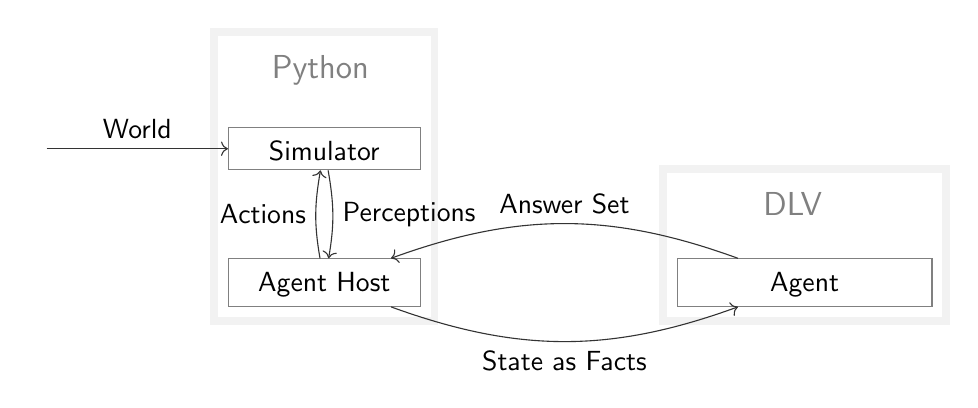
\begin{tikzpicture}[
			node distance=1cm and 5mm,
			every node/.style={font=\sffamily},
			title/.style={font=\color{black!50}\sffamily},
			typetag/.style={rectangle, draw=black!50, font=\sffamily, anchor=west, text height=3mm, align=center}
			]
			
			\node (lp) at (0, -1cm) {};
			\node (as) at (0, -3.2cm) {};
			
			\node (gl) at (3.6cm, 0) [align=center, text width=2.1cm, title] { \large Python };
			
			\node (par) [below=of gl.west, text width=22mm, typetag] { Simulator };
			\node (gro) [below=1.7cm of par.west, text width=22mm, typetag] { Agent Host };
			
			\node (g) [draw=gray!10, line width=1mm, inner sep=5pt, fit={(gl) (par) (gro)}] {};
			
			\node (sl) at (9.6cm, -1.7cm) [align=center, text width=2.7cm, title] { \large DLV };
			
			\node (ngs) [below=of sl.west, text width=3cm, typetag] { Agent };
			
			\node (s) [draw=gray!10, line width=1mm, inner sep=5pt, fit={(sl) (ngs)}] {};
			
			\draw [->, draw=black!80] (gro) to [out=340, in=200] node [midway, below] {State as Facts} (ngs);
			\draw [->, draw=black!80] (ngs) to [out=160, in=20] node [midway, above] {Answer Set} (gro);
			
			\draw [->, draw=black!80] (par) to [out=280, in=80] node [midway, right] {Perceptions} (gro);
			\draw [<-, draw=black!80] (par) to [out=260, in=100] node [midway, left] {Actions} (gro);
			
			\draw [->, draw=black!80] (lp) -- (par) node [midway, above] {World};
			\end{tikzpicture}
	
  		\caption{Architecture }
  	\end{figure}
	
  \end{frame}


  \section{Evaluation}
  
  \begin{frame}{Perfect agent}
    Performance of the agent compared against a \alert{perfect} agent.
    \begin{itemize}
      \item \alert{Omniscience}, i.e. total knowledge of the world 
      \item Optimal solution as shortest path over the action graph
      \item Score of this agent taken as reference for a dungeon
    \end{itemize}
  \end{frame}

  \begin{frame}{The Test Suite}
    %Powered by \alert{PyTest}.

  \end{frame}

  \section{Conclusion}

  \begin{frame}{Possible Improvements}
      % TODO: I think this can be skipped, if we do a good job.
  \end{frame}

  \begin{frame}{Conclusion}
  \end{frame}

  \begin{frame}[standout]
    Thank you!
  \end{frame}

\end{document}
